\documentclass[reprint,english,notitlepage,aps,nobalancelastpage,nofootinbib]{revtex4-1}
\usepackage[utf8]{inputenc}
\usepackage[english]{babel}
\usepackage{physics,amssymb}
\usepackage{graphicx}
\usepackage{xcolor}
\usepackage{hyperref}
\usepackage{tikz}
\usepackage{listings}
\usepackage{subfigure}
\usepackage{amsmath,mathtools}
\usepackage{amsbsy}
\usepackage{enumitem}
\usepackage{bbold}

\graphicspath{{../plots/}}

\hypersetup{
    colorlinks,
    linkcolor={red!50!black},
    citecolor={blue!50!black},
    urlcolor={blue!80!black}}

\lstset{
	inputpath=,
	backgroundcolor=\color{white!88!black},
	basicstyle={\ttfamily\scriptsize},
	commentstyle=\color{magenta},
	language=Python,
	morekeywords={True,False},
	tabsize=4,
	stringstyle=\color{green!55!black},
	frame=single,
	keywordstyle=\color{blue},
	showstringspaces=false,
	columns=fullflexible,
	keepspaces=true}


\newcommand{\closed}[1]{\left(#1\right)}
\newcommand{\bracket}[1]{\left[#1\right]}

\newcommand{\tmdv}[4]{\closed{\pdv{#1}{#2}}_{#3,#4}}
\newcommand{\jacobian}[2]{\pdv{(#1)}{(#2)}}
\renewcommand{\d}{\mathrm{d}}
\newcommand{\sumstate}{\sum_{\{\sigma_j\}}}
\newcommand{\prodstate}{\prod_{i=0}^{L-1}}
\newcommand{\ebj}{e^{\beta J}}
\newcommand{\T}[1]{T_{\sigma_{#1},\sigma_{#1 + 1}}}
\renewcommand{\l}{\lambda}
\newcommand{\mj}{m_j}

\begin{document}
\begin{center}
\title{\Huge FYS4130 - Oblig 2}
\author{\large Vetle A. Vikenes}
\date{\today}
\noaffiliation


\maketitle
\end{center}
\onecolumngrid

All code used in this oblig can be found on my Github: \url{https://github.com/Vikenes/FYS4130}
\\
\section*{\large Task 1 - Transfer Matrices}

\subsection*{a) Partition function and average internal energy}

We consider a 1D spin chain of length $L$ with periodic boundary conditions. The Hamiltonian of the system given as  
\begin{align} \label{eq:Hamiltonian}
	H &= -J \sum_{i=0}^{L-1} \delta_{\sigma_i,\sigma_{i+1}},
\end{align}

where $\sigma_i=\{0,\,1,\,2\}$ denotes the spin at site $i$ and $J>0$.    

The order parameter, $m$, and local magnetization, $m_j$, is given by
\begin{align}
	m &\equiv \frac{1}{N} \sum_{j=0}^{N-1} m_j \label{eq:order parameter}  \\ 
	\text{where}\quad m_j &\equiv e^{i(2\pi/3)\sigma_j} \label{eq:magnetization}
\end{align}

To calculate the partition function, we begin by inserting the expression for the Hamiltonian and write the sum in the exponent in terms of products. 
\begin{align*}
	Z &= \sum_{\{\sigma_j\}} e^{-\beta H} = \sumstate e^{\beta J \sum_{i=0}^{L-1} \delta_{\sigma_i,\sigma_{i+1}}} = \sumstate \prod_{i=0}^{L-1} e^{\beta J \delta_{\sigma_i,\sigma_{i+1}}}
\end{align*}

The exponential can be written in terms of transfer matrices representing the different values of the exponential for different spin states. Letting $\sigma_i$ and $\sigma_{i+1}$ govern the row and column, respectively, the transfer matrix becomes 

\begin{align} \label{eq:transfer_matrix}
	T_{\sigma_i,\sigma_{i+1}} &= 
	\begin{pmatrix}
		e^{\beta J} & 1 & 1 \\
		1 & \ebj & 1 \\
		1 & 1 & \ebj
	\end{pmatrix}.
\end{align}

The transfer matrix will thus look identical for different values of $\sigma_i$, so taking the product between different ones, results in a transfer matrix raised to a certain power.  

\begin{align*}
	Z &= \sumstate \prodstate \T{j} = \sumstate T_{\sigma_0,\sigma_1} T_{\sigma_1,\sigma_2}\cdots T_{\sigma_{L-1},\sigma_0} 
\end{align*}
where we invoked the periodicity, $\sigma_L=\sigma_0$, in the last line. This means that we're summing over repeated indices, and the sum can be carried out by taking the trace of the resulting matrix products. To calculate the product of the matrices, we start by diagonalizing it, writing it as $T=PDP^{-1}$, with

\begin{align*}
	P &= 
	\begin{pmatrix*}[r]
		-1 & -1 & 1 \\ 
		0  & 1  & 1 \\ 
		1  & 0  & 1 
	\end{pmatrix*} ,\quad D = \begin{pmatrix*}[r]
		\lambda_1 & 0 & 0 \\ 
		0 & \lambda_2 & 0 \\
		0 & 0 & \lambda_3 
	\end{pmatrix*},\quad
	P^{-1} = \frac{1}{3} \begin{pmatrix*}[r]
		-1 & -1 & 2 \\ 
		-1 & 2  & -1 \\ 
		1  & 1  & 1
	\end{pmatrix*},
\end{align*}

where the eigenvalues of $T$ are 
\begin{align*}
	\lambda_1 &= \ebj-1 \\ 
	\lambda_2 &= \ebj-1 \\ 
	\lambda_3 &= \ebj+2
\end{align*}

Since the summation of transfer matrices in our expression for $Z$ is over repeated indices, the sum corresponds to taking the trace of the matrix, so our expression for $Z$ becomes 

\begin{align*}
	Z &= \Tr(T_{\sigma_0,\sigma_0}^N) = \Tr(PDP^{-1}PDP^{-1}\cdots PDP^{-1}) \\ 
	&=Tr(P D^L P^{-1})= \Tr(D^L) = \lambda_1^L + \lambda_2^L + \lambda_3^L,
\end{align*}
where we used the cyclic property of the trace to eliminate the final $P$ and $P^{-1}$. 

Inserting the eigenvalues, we finally arrive at 
\begin{align}
	Z &= 2\closed{\ebj - 1}^L + \closed{\ebj+2}^L \label{eq:partition_function}
\end{align}

We will now use equation \eqref{eq:partition_function} to calculate the average total energy, $U$, which is obtained through the following partial derivative  

\begin{align*}
	U &= \pdv{(\beta F)}{\beta}.
\end{align*}

The product $\beta F$ is gotten from the negative logarithm of $Z$, and is thus 

\begin{align*}
	\beta F = -\ln Z = -\ln\bracket{2(\ebj-1)^L + (\ebj+2)^L}.
\end{align*}

Differentiating this with respect to $\beta$, we get

\begin{align}
	U &= -\frac{2L(\ebj-1)^{L-1} J\ebj + L(\ebj+2)^{L-1}J\ebj}{2(\ebj-1)^L + (\ebj+2)^L} \nonumber \\[10pt]
	& = -LJ\ebj \cdot \frac{2(\ebj-1)^{L-1}+(\ebj+2)^{L-1}}{2(\ebj-1)^L + (\ebj+2)^L} \label{eq:avg_tot_en}
\end{align}

Now, we want to find an approximate expression for $U$ valid for low and high temperatures. Rather than working with $U$ directly, we will instead rewrite the partition function in a way that allows us to simplify it. 
\begin{align*}
	Z = 2\l_1^L + \l_3^L = \l_3^L\bracket{2\closed{\frac{\l_1}{\l_3}}^L+1},
\end{align*} 
where a factor $\l_3$ has been taken outside the brackets, since $\l_3>\l_1$. For large values of $L$ we can now see that the behaviour of $Z$ is restricted to two separate cases, corresponding to small and large values of $\beta$. 

If $\beta$ is very large, the constant terms of the eigenvalues become negligible, so we get $\l_1/\l_3\approx1$. In this case we get $Z\approx 3\l_3^L$. If, on the other hand, $\beta$ is small we have $\l_1\ll \l_3 \implies (\l_1/\l_3)^L \to 0$. The expression for $Z$ is then $Z\approx \l_3^L$.  

Our two expressions for $Z$ differs only by a constant factor. Upon differentating the logarithm of $Z$ this constant vanishes, so our approximate expression for $U$ becomes       
\begin{align*}
	U&=-\pdv{\beta}\ln Z \approx -\pdv{\beta} L \ln \l_3 = -L \pdv{\beta}\ln (\ebj+2) \\ 
	&= -\frac{LJ}{1+2 e^{-\beta J}}, 
\end{align*}
which is valid at both high and low values of $T$. Computing the two limiting cases, we find  

\begin{align*}
	\lim_{\beta\to\infty} U = -LJ,\:\:\text{and}\quad \lim_{\beta\to0} U = -\frac{LJ}{3}
\end{align*}
Using WolframAlpha, we get the same results for the two limits of $U$ from equation \eqref{eq:avg_tot_en}, and therefore conclude that our approximation is reasonable. 

For the physical interpretation, the low temperature limit corresponds to our model having its minimum energy, where all the spins are aligned. In the high temperature limit we have disordered spin states, uniformly distributed among the three possible values of $\sigma_j$. The probability of neighbouring spins being aligned in this case is then $1/3$, such that the Hamiltonian only yields a non-zero term in its sum for $1/3$ of all the configurations.


\subsection*{b) - Average magnetization}

We now want to show that the average magnetization, $\expval{m}$, equals zero at all temperatures. We can express the average magnetization as 
\begin{align*}
	\expval{m} = \frac{1}{N} \sum_{i=0}^{N-1}\expval{m_j},
\end{align*}
and we can now compute $\expval{\mj}$, and we start by inserting transfer matrices, as we did before.  

\begin{align*}
	\expval{m_j} &= \frac{1}{Z} \sumstate \mj e^{-\beta H} = \frac{1}{Z} \sumstate e^{i(2\pi/3)\sigma_j} \prodstate \T{j}
\end{align*} 

Summing all the spins from $\sigma_1$ up to $\sigma_{j-1}$ yields a factor of $T_{\sigma_0,\sigma_j}^j$ at the beginning as well as a similar factor raised to the power $L-j$ at the end, so $\expval{\mj}$ can therefore be written as   

\begin{align*} 
	\expval{\mj} &= \frac{1}{Z} \sum_{\sigma_0} \sum_{\sigma_j} T_{\sigma_0,\sigma_j}^j e^{i(2\pi/3)\sigma_j} \,T_{\sigma_j,\sigma_0}^{L-j}
\end{align*}
To carry out the sum, we now use that we sum over repeated indices and we thus have to compute the trace of the resulting matrix. Since the diagonal elements of the original transfer matrix in equation \eqref{eq:transfer_matrix} are identical, the diagonal elements of the same matrix raised to a certain power will also be identical. This leaves us with the same factor in front of the three different exponential terms, and we get 

\begin{align*}
	\expval{\mj} &= \frac{1}{Z} \closed{T_{0,0}^j\,T_{0,0}^{L-j} + e^{i2\pi/3} \,T_{1,1}^j\,T_{1,1}^{L-j} + e^{-i2\pi/3}\,T_{2,2}^j\,T_{2,2}^{L-j}} \\ 
	&= \frac{1}{Z} \closed{1 + e^{i2\pi/3} + e^{-i2\pi/3}} 3\,T_{0,0}^{j} \, T_{0,0}^{L-j} \\ 
	&= 0.
\end{align*}  
With $\expval{\mj}=0$ we then get $\expval{m}=\sum \expval{\mj}/N=0$, which is what we wanted to show.


\subsection*{c) - Correlation function}
The correlation function is defined as 
\begin{align} \label{eq:corr_func}
	C(r) &\equiv \expval{m_0^* m_r} - \expval{m_0^*}\expval{m_r}.
\end{align}
Having already found that $\expval{\mj}=0$, the last term in equation \eqref{eq:corr_func} vanishes, and we're left with the quantity $\expval{m_0^* m_r}$, which we can write in terms of exponentials as 

\begin{align*}
	\expval{m_0^* m_r} &= \expval{e^{i(2\pi/3)(\sigma_r - \sigma_0)}}.
\end{align*}

We follow the same procedure as before, writing out all sums except for the ones over $\sigma_0$ and $\sigma_r$ this time. 

\begin{align*}
	\expval{m_0^* m_r} &= \frac{1}{Z} \sumstate m_0^* m_r \, \prodstate \T{i} = \frac{1}{Z} \sum_{\sigma_0} \sum_{\sigma_r} e^{i\frac{2\pi}{3}(\sigma_r-\sigma_0)} T_{\sigma_0,\sigma_r}^{r} \, T_{\sigma_r,\sigma_0}^{L-r} 
\end{align*}

Now, the exponential term can be written as a matrix with indices $(\sigma_r,\sigma_0)$, meaning that we can't simply compute the trace in this case. Before computing anything, we will first consider the general form of the transfer matrices raised to a certain power. 

Using the diagonalization $T=PDP^{-1}$, we write the general expression for $T_{i,j}^k=(PD^k P^{-1})_{i,j}$ gotten from the matrix multiplication. The resulting matrix will have identical terms on the diagonal, as well as identical terms on the off-diagnoal. These terms are given in equation \eqref{eq:T_power}  

\begin{align} \label{eq:T_power}
	T_{i,j}^k = \frac{1}{3}\begin{cases}
		2(\ebj-1)^k + (\ebj+2)^k \quad &\mathrm{for}\; i=j \\ 
		-(\ebj-1)^k + (\ebj+2)^k \quad &\mathrm{for}\; i\neq j
	\end{cases}
\end{align}

When we sum over different spin combinations, there will be three terms corresponding the case of equal indices in equation \eqref{eq:T_power}, where the exponent simply contributes a factor $1$. On the off-diagonal, three terms will have a common factor of $e^{i(2\pi/3)}$. The same three terms will also have a common factor of $e^{-i(2\pi/3)}$, since $T_{i,j}=T_{j,i}$. For the off-diagonal terms we are then left with three terms having a common factor $e^{i(2\pi/3)} + e^{-i(2\pi/3)}=-1$. 

To simplify the writing, we write $T_{i=i}$ for diagonal terms and $T_{i\neq j}$ for off-diagonal terms.

\begin{align*}
	\expval{m_0^* m_r} =& \frac{1}{Z} \Big[ 3\, T_{i=i}^r T_{i=i}^{L-r} - 3T_{i\neq j}^r T_{i\neq j}^{L-r} \Big] \\ 
	=& \frac{3}{Z} \Bigg( \frac{1}{3} \Big[ 2(\ebj-1)^r + (\ebj+2)^r \Big]\cdot \frac{1}{3} \Big[2(\ebj-1)^{L-r} + (\ebj+2)^{L-r} \Big] \\ 
	&\quad\:\: -\frac{1}{3}\Big[(\ebj+2)^r-(\ebj-1)^r \Big] \cdot \frac{1}{3}\Big[(\ebj+2)^{L-r}-(\ebj-1)^{L-r} \Big]  \Bigg) \\
	=& \frac{1}{Z} \cdot \frac{1}{3} \Bigg( 4(\ebj-1)^L + (\ebj+2)^L + 2(\ebj-1)^r (\ebj+2)^{L-r} + 2 (\ebj+2)^r (\ebj-1)^{L-r}  \\
	& \qquad\quad - \Big[(\ebj-1)^L + (\ebj+2)^L - (\ebj-1)^r (\ebj+2)^{L-r} - (\ebj+2)^r (\ebj-1)^{L-r} \Big] \Bigg)
\end{align*}
The two terms $(\ebj+2)^L$ will now cancel each other out, while the remaining terms will all have a factor $3$ canceling the factor $1/3$ in front. Finally, writing out the partition function, our final expression for the correlation function becomes 

\begin{align} \label{eq:corr_func_result}
	C(r) &= \frac{(\ebj-1)^L + (\ebj-1)^r (\ebj+2)^{L-r} + (\ebj-1)^{L-r} (\ebj+2)^r}{2(\ebj-1)^L + (\ebj+2)^L}
\end{align}



Now we want to find the limiting result of $C(r)$ for $L\to\infty$. This is most easily done by resorting to WolframAlpha, from which we get that
\begin{align*}
	\lim_{L\to\infty} C(r) = \closed{\frac{\ebj-1}{\ebj+2}}^r = \closed{\frac{\l_1}{\l_3}}^r
\end{align*}
The limiting case is still a function of $r$, which is desired, since two spins separated by a short distance will still be correlated no matter how long the overall chain is. With $\l_1<\l_3$ we also get that the longer the separation between spins, the less they are correlated. 

For the case $T=0$, we let WolframAlpha compute the limit as $\beta\to\infty$ and get 
\begin{align*}
	\lim_{T\to0} C(r) = 1,
\end{align*}
implying that there is a perfect correlation between all spins. This coincides with the fact that all the spins are alligned when $T=0$, as discussed in 1a). 

\section*{\large Task 2 - Monte Carlo Simulations}


\begin{figure}[h!]
	\centering
	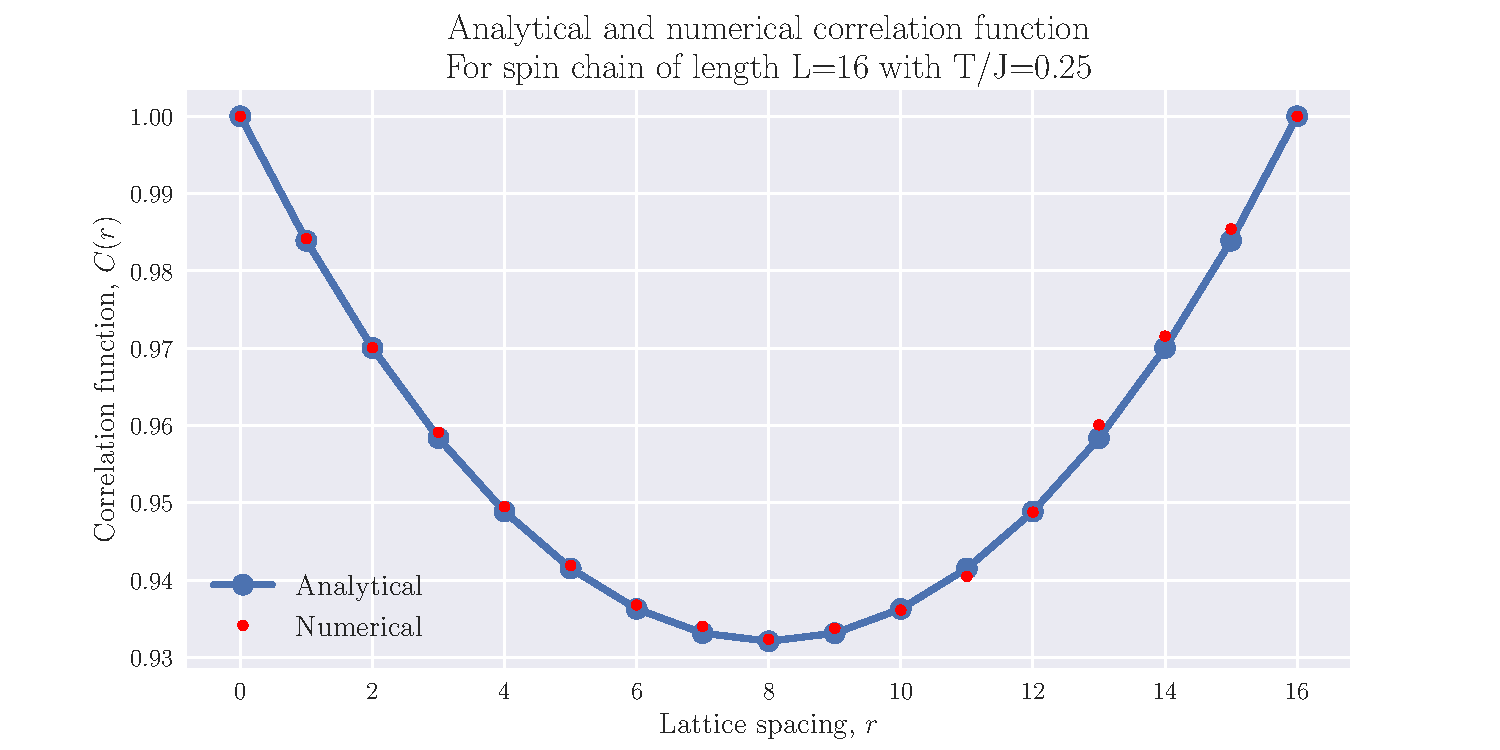
\includegraphics[width=0.7\linewidth]{correlation1D_025.pdf}
	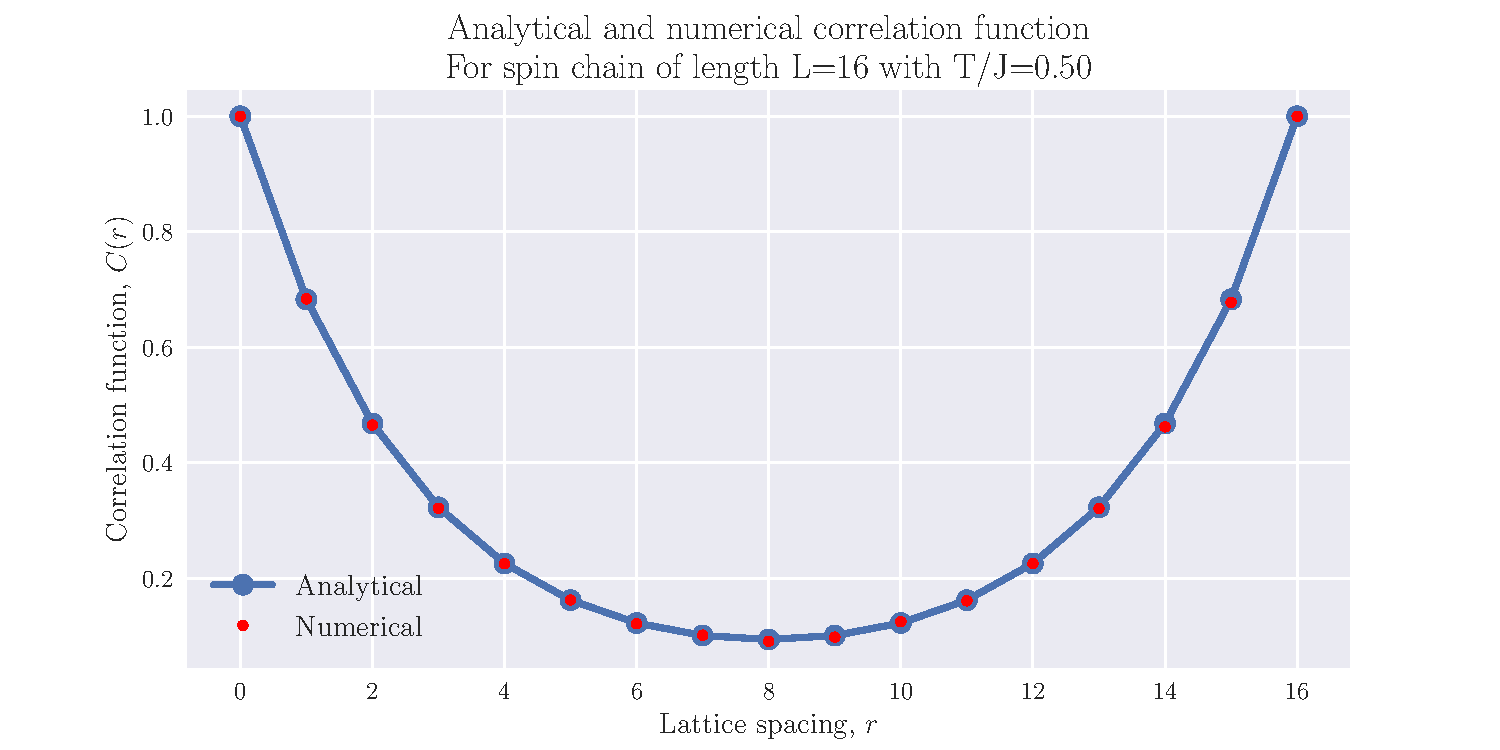
\includegraphics[width=0.7\linewidth]{correlation1D_05.pdf}
	\caption{Correlation}
	\label{fig:correlation}
\end{figure}


\end{document}
